The simulations are based on a realistic network topology were run in 
 a 1.60 GHz Quad Core machine with 16 GBytes of available RAM.

In order to run the test Ubuntu Operating system was install with WSL2 ( Ubuntu running on Windows Kernel).
 
\textbf{In our case we had the following:} 


\begin{figure}[h]
    \centering
    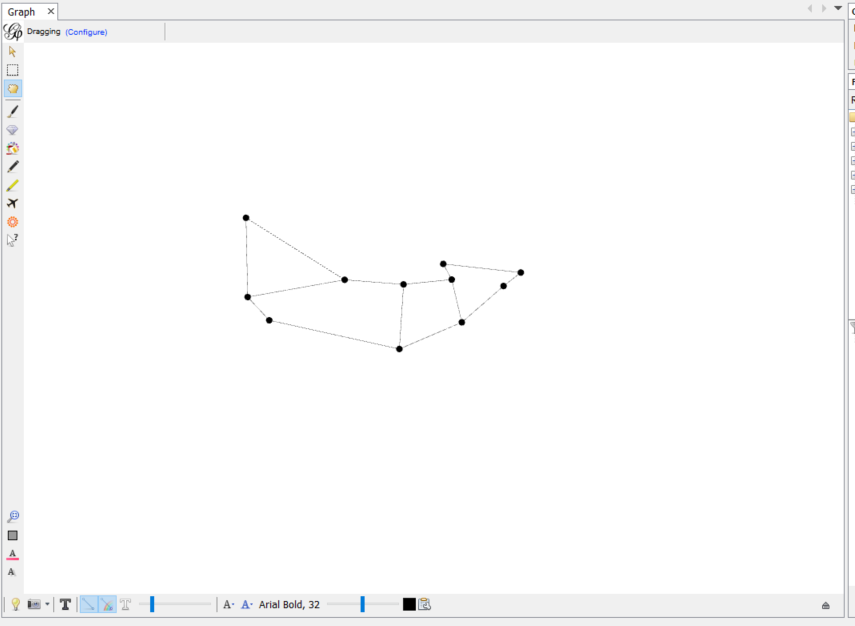
\includegraphics[width=1\textwidth]{abilene_gephi}
    \caption{Abilene graphml as viewed in Gephi}
    \label{fig:abilene_gephi}
\end{figure}

\begin{figure}[h]
    \centering
    \includegraphics[width=1\textwidth]{input_graph_data}
    \caption{Abilene network topology data(1)}
    \label{fig:input_graph_data}
\end{figure}

\begin{figure}[h]
    \centering
    \includegraphics[width=1\textwidth]{input_graph_edges}
    \caption{Abilene network topology data(2)}
    \label{fig:input_graph_edges}
\end{figure}

\begin{figure}[h]
    \centering
    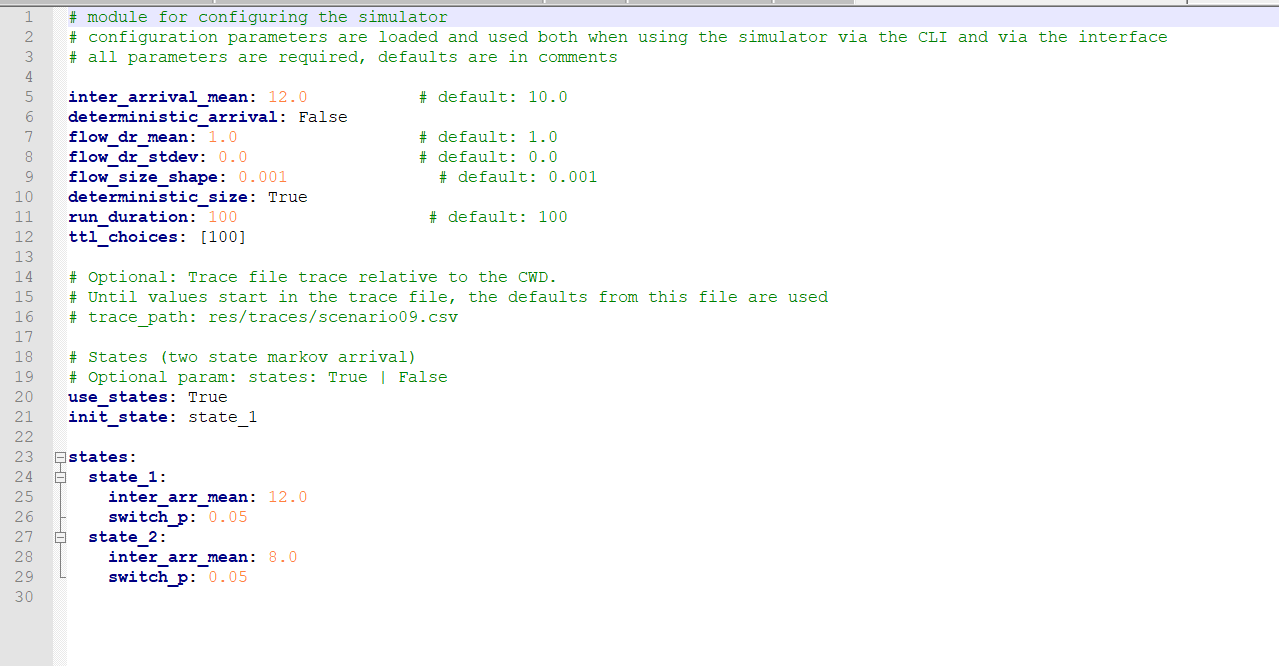
\includegraphics[width=1\textwidth]{simulation_config}
    \caption{Simulation configuration}
    \label{fig:simulation_config}
\end{figure}
\begin{figure}[h]
    \centering
    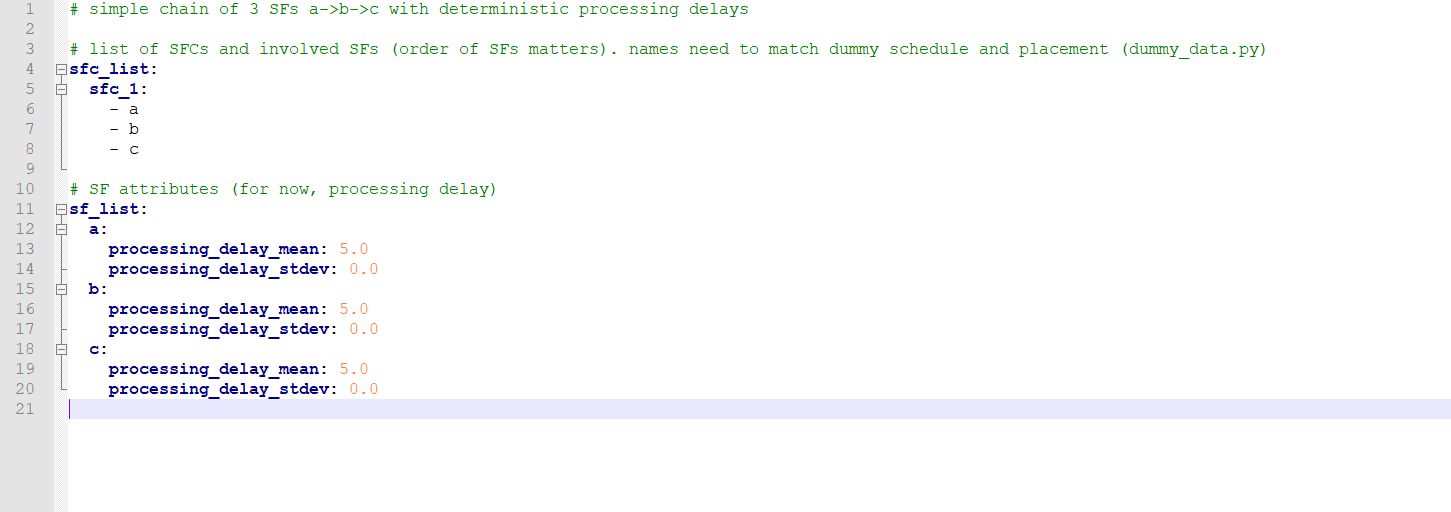
\includegraphics[width=1\textwidth]{SF_chaing}
    \caption{SFCs simulation configuration}
    \label{fig:SF_chaing}
\end{figure}
